% Number 980
% CAPMG NAPM  Units 
% Changing v from a graph - graphical
% JG

% Watermark
\AddToShipoutPicture*{\BackgroundPic}

\addtocounter {ProbNum} {1}

\begin{floatingfigure}[r]{.44\textwidth}
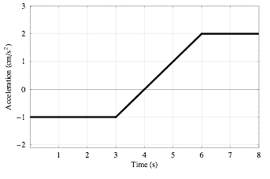
\includegraphics[scale=.95]{/Users/jgates/desktop/latex/pics/agraph1}
\end{floatingfigure}
 
{\bf \Large{\arabic{ProbNum}}} The acceleration graph for a cart moving along a straight-line track is shown below.\bigskip
       
Calculate the change in velocity over the first 3 seconds of motion.   \paragraph{}
\noindent
\vfill

Calculate the change in velocity over the entire 8 seconds of motion.    
\vfill

Given that the cart starts with an initial velocity of ${+2~\tfrac{m}{s}}$, plot the velocity graph for this motion.  (Yep, this is a bit tricky... go for it! Break the graph into useful parts.) 
\begin{center}
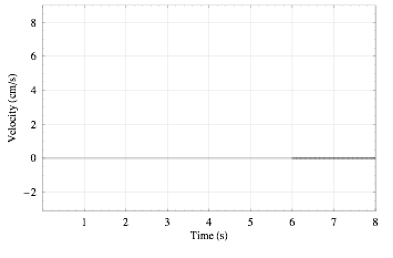
\includegraphics[scale=.7]{/Users/jgates/desktop/latex/pics/vgraph8}
\end{center}

Describe the motion of the object in words, based on the velocity graph that you drew.
\vfill



\newpage